\subsection{Propuestas}
Se propone utilizar arquitecturas \aclink{RAG} para mejorar la precisión, ofreciendo al modelo información sobre la generación de consultas \aclink{JQL}. La idea detrás de esto es que, al tener un modelo de recuperación que pueda acceder a una base de conocimiento, el modelo de generación pueda generar respuestas más precisas y acordes al contexto proporcionado. Además, se propone un nuevo conjunto de datos:

Si bien el conjunto de datos inicial era robusto, se ha propuesto un nuevo conjunto, de 100 preguntas, que busca, no solo tener más datos, sino hacerlos más diversos y cambiar en cierto modo las preguntas para cubrir el máximo número de casos posible. Este conjunto de datos se ha pensado durante el desarrollo y las diferentes pruebas lanzadas y también se ha usado como apoyo un dataset existente en \textit{Hugging Face}~\cite{datasetHF}.

A continuación, se describirán las distintas alternativas propuestas para mejorar la precisión del modelo JiraGPT Next.

\subsubsection{Ontología}
Durante el inicio de este trabajo se consultaron artículos como \textit{Sequeda et al.}~\cite{sequeda2023benchmark}, que exploraban la posibilidad de utilizar ontologías en el prompt para mejorar la interpretación de los datos y la generación de consultas SQL, logrando resultados prometedores. Partiendo de esta idea, se propone entonces crear una ontología que represente las reglas que existen en las consultas JQL. La información que se pretende representar en la ontología se ha extraído directamente de la documentación oficial de JIRA, brindada por Atlassian, donde se detallan las reglas que se deben seguir para la creación de consultas JQL~\cite{jiradocs}. Esta ontología serviría para interpretar las reglas que hay que seguir al generar consultas JQL, además, consta de ejemplos en cada una de las clases definidas, que ayuda a comprender mejor el funcionamiento de las reglas.

La ontología se ha desarrollado siguiendo el estándar \textit{Web Ontology Language} (OWL), que es un lenguaje de marcado semántico para publicar y compartir ontologías en la web. OWL es desarrollado por el \textit{World Wide Web Consortium} (W3C) y es una extensión de \textit{Resource Description Framework} (RDF).

Durante esta parte, se considera una ejecución del benchmark como \textit{baseline} para comparar los resultados obtenidos con la ontología y sin ella. Esta primera ejecución se realizaría inyectando el archivo entero de la ontología en el prompt, de manera que el modelo pueda acceder a la información de la ontología y utilizarla para generar consultas más precisas.
Esta aproximación podría presentar resultados que, a priori, parecieran prometedores. Sin embargo, de cara al coste de inyectar un prompt tan grande, no es viable en un entorno de producción. Por ello, se propone una recuperación de información de la ontología dado un campo relevante para la pregunta del usuario. El diagrama en la siguiente figura muestra cómo será la interacción entre el modelo y la ontología.

\begin{figure}[H]
    \centering
    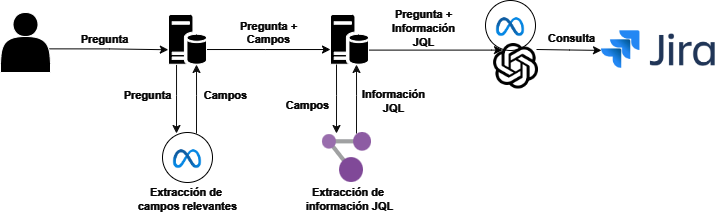
\includegraphics[width=0.95\textwidth]{images/rag_ontologia.png}
    \caption{Diagrama de RAG con ontología}\label{fig:ontologia}
\end{figure}
Si bien una ontología es una manera de representar un espacio de conocimiento, la documentación de JIRA no presenta una estructura demasiado compleja que representar con la semántica de una ontología. Podría considerarse que, por ende, no es realmente necesario el uso de una ontología para representar las reglas de JQL. Sin embargo, tras lo realizado en este trabajo, no sería complicado utilizar otra ontología que reuniese información más compleja y permitiese explotar la semántica de la ontología para mejorar la generación de consultas JQL.

\newpage
\subsubsection{Embeddings}
De igual manera que en el diseño de la ontología, se propone capturar en esta base de datos vectorial la documentación oficial de JIRA. Esta base de conocimiento prueba a guardar los embeddings de los diferentes descripciones dentro de la documentación. La información que se ha considerado relevante ha sido cada campo/operador/función y sus respectivos ejemplos. De esta manera, dada una pregunta se podrían obtener los embeddings de las palabras y compararlas con los embeddings de la base de datos, de manera que el modelo obtenga ejemplos de campos relevantes para la pregunta del usuario.

Para capturar toda la información de la documentación se ha diseñado un programa en Python que realiza técnicas de \textit{web scraping} y recorre las entradas de la documentación extrayendo de las tablas los ejemplos. Una vez hecho esto, se guarda en un archivo de texto que será dividido en diferentes partes para ser procesado por el modelo de embeddings.

Teniendo la pregunta del usuario, se ha de traducir al inglés, ya que la documentación oficial está en inglés y dada una pregunta en castellano la recuperación de información de los embeddings no sería efectiva. Para traducir la pregunta, se utiliza GPT-4o y, dada la pregunta traducida, se hace una búsqueda en la base de datos vectorial, obteniendo los ejemplos más relevantes para la pregunta dada. Esta información se inyecta en el prompt para que el modelo pueda generar una respuesta más precisa. El diagrama en la siguiente figura muestra cómo será la interacción entre el modelo y la base de datos vectorial.

\begin{figure}[H]
    \centering
    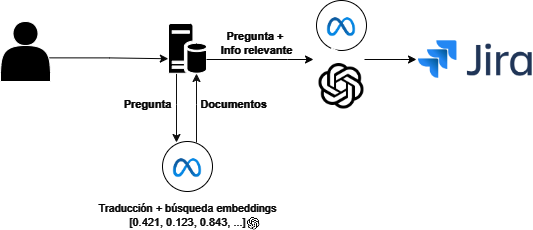
\includegraphics[width=0.95\textwidth]{images/rag_embeddings.png}
    \caption{Diagrama de RAG con embeddings}\label{fig:embeddings}
\end{figure}

\newpage
\subsubsection{Grafos de conocimiento}
Como última propuesta para el trabajo, se ha planteado el uso de grafos de conocimiento para tratar de guiar al modelo en la estructura de la información contenida en la plataforma JIRA de LKS Next-GobTech. La idea detrás de esta propuesta es que, dada la información de Jira en forma de grafo, el modelo podría ser capaz de inferir cómo es la estructura de información de la plataforma Jira de LKS Next-GobTech y generar respuestas que sean más acordes a lo que se busca. Para esto, se ha de crear un grafo de conocimiento que contenga la información de Jira de cada proyecto que tenga activo LKS Next-GobTech, por lo que se ha de crear un programa que sea capaz de transformar esa información en un grafo y se pueda ejecutar de manera periódica, con el fin de que el grafo esté actualizado con la información real que se almacena en Jira.

El flujo sería el representado en la figura siguiente, donde se muestra cómo, dada una pregunta de un usuario, se extrae información del grafo de conocimiento que se inyectaría en el prompt para que el modelo pueda generar una respuesta con más contexto.

\begin{figure}[H]
    \centering
    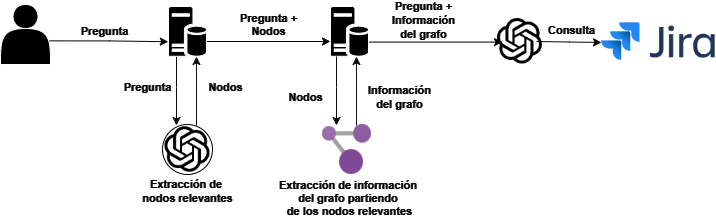
\includegraphics[width=0.95\textwidth]{images/rag_grafo.png}
    \caption{Diagrama de RAG con grafos de conocimiento}\label{fig:kg}
\end{figure}
